\section{Background}

Our work focuses on energy saving in cloud storage systems through the use of
block level caching mechanisms. We use DM-Cache as the block level caching
mechanism to evaluate our work on as it is freely available as a Linux kernel
module and is currently in use in many cloud storage systems such as Facebook's
FlashCache which is based on the implementation of DM-Cache \cite{flashcache}.

\subsection{DM-Cache}

\begin{figure}
  \caption{Architecture of DM-Cache}
  \centering 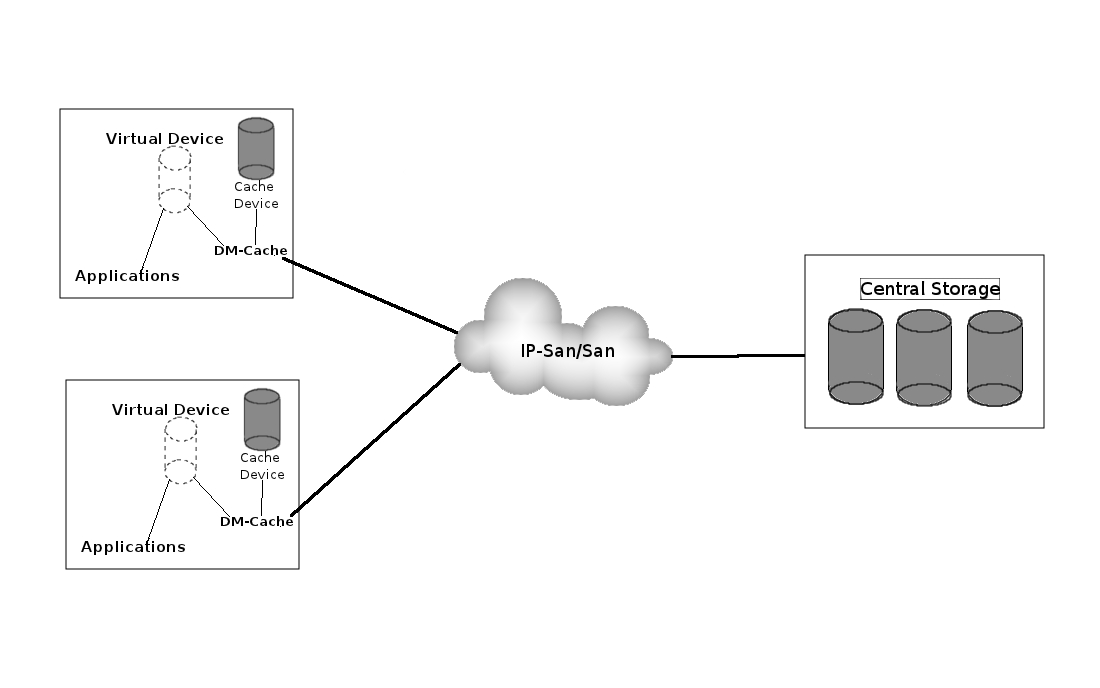
\includegraphics[width=0.5\textwidth]{dm-cache_diagram.jpg}
  \label{fig:dm-cache}
\end{figure}

DM-Cache is a block-level caching mechanism implemented as a module in the Linux
kernel \cite{DM-Cache}. It allows for specification of a local SSD as a cache
device where recently used blocks can be stored for faster access time. It
supports both write-back and write-through functionality for handling cached
data. Figure~\ref{fig:dm-cache} shows the architecture of DM-Cache.

The purpose of DM-Cache is to cache recently used blocks on local storage
instead of retrieving them from some external storage source. This helps to
alleviate network bandwidth issues as well as reduce response times and save
power by issuing less requests to the storage node.

The current implementation of DM-Cache uses a hash table that maps logical block
addresses to entries within the hash table and evictions are done when two block
addresses map to the same entry but contain different data. This eviction scheme
does not take into account most recently used blocks and it also does not make
any attempt to pre-fetch any other blocks.
